%signal acquisition
%included in skripsie.tex

\section{Overview}

The signal acquisition module (SAM) captures all signals present on
the scalp surface and passes it on to the low--level signal processing
module's differential inputs. The signal acquisition module is
implemented using a set of active electrodes mounted on a removable
head--band.


The design and implementation of SAM entails the realization of the
physical electrodes as well as the electronic implementation of the
active electrode circuitry. The positioning of the device on the
cranium and the corresponding placement of the electrode's contact
surfaces is dependent on the design of the SAM container or
head--band. While all aspects of SAM design and implementation is
explored in some detail special consideration is given to noise
containment and elimination.


The goal of replacing passive electrodes with active devices implies a
redesign or enhancement of the standard passive electrodes as well as
their method of application. The traditional methods of reducing
electrode noise and motion artifacts are incompatible with the
high--level requirements of user friendliness and ease of use. 


Passive electrodes are the main injection point for external
interference into a EEG capturing system. By using active circuitry to
address the problems associated with traditional EEG electrodes the
noise and interference problems are addressed and the system's
usability enhanced.

\section{SAM design specification}

The signal acquisition module is required to produce a EEG signal of
at least comparative quality than that of current silver or gold
electrodes. The signal quality is defined in terms of noise present in
the output signal from the signal acquisition module. It is inevitable
that the active components of the active electrode will inject more
noise into the system that normal passive electrodes will. The
benefits derived from using a AE in terms of interference reduction
and greater CMRR due to reduced DC offset levels at the
instrumentation amplifiers input must compensate for the noise
injected by the active components.


The SAM submodule must also circumvent the current usability problems
associated with traditional electrodes.


The SAM must be able to deliver a low-noise EEG signal to the the
low-level signal processing module's (Chapter~\vref{chap:sa})
differential input stage. The EEG signal must be spectrally unaltered
in the band of interest (0.1~Hz~--~35~Hz) with a flat frequency
response within $\pm$0.5~dB of the source signal.


The SAM must also comply to the high--level design constraints set in
Table~\vref{table:hl-design-contraints}, that is a maximum permissible
application and adjust time of 10~s, a maximum removal time of 5~s and
no skin preparation.

The SAM design specification is logically sub-dived into a active
electrode and active electrode container specification:
\begin{itemize}
	\item{Active Electrode design specification} 
		\begin{itemize} 

			\item{The active electrode electronic design. Signal to
			noise ratio values, input and output impedances and the
			AE's transfer function are specified.}

			\item{The active electrode physical design dealing with
			physical aspects of the active electrode parameters including
			contact area and manufacturing processes.}

		\end{itemize}
	\item{Active Electrode container specification}
	
		\begin{itemize}
			\item{Specification of the montage protocol, and the degree of
			adjustment variability}
		\end{itemize}
\end{itemize}


Separating the design allows for the substitution of either designs or
subsequent implementations by another design or implementation for
comparative analysis. For example the contact area of the physical
electrode may be varied or the metal used in manufacturing may be
changed without changing the electronic design, and vice versa.


\subsection{AE electronic design specification}

In order to effectively develop the AE electronic design specification
cognizance must be taken of noise and interference problems
experienced when using traditional passive electrodes.

\subsubsection{Noise and interference analyses of passive electrodes}
\label{section:passive-analyses}
\begin{figure}[htb]
	\begin{center}
	\psfrag{eeg}{$e_{EEG}$}
	\psfrag{re}{$R_e$} 
	\psfrag{rc}{$R_c$} 
	\psfrag{cc}{$C_c$}
	\psfrag{rsg}[][]{$R_{sg}$}
	\psfrag{rsg}[][]{\colorbox{white}{$R_{sg}$}}
	\psfrag{electrolyte}{Electrolyte}
	\psfrag{movement}{Movement}  
	\psfrag{emi}[][]{EM interference}
	\psfrag{fields}{fields}  
	\psfrag{stratum granulosum}{\em stratum granulosum \em}  
	\psfrag{soft tissue}{Soft tissue}
	\psfrag{cranium}{Cranium}
	\psfrag{Brain}{Brain}
	\psfrag{metal}{Metal}
	\psfrag{contaminant}{Contaminant}
	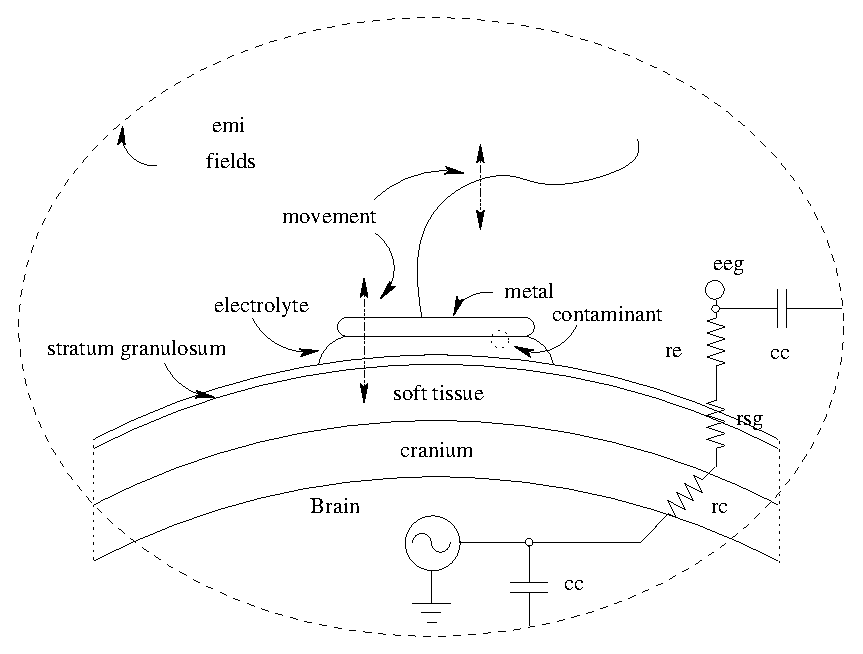
\includegraphics[width=\textwidth]{electrode-noise.eps}
	\caption{Passive electrode noise sources}
	\label{fig:electrode-noise} 
	\end{center}
\end{figure}


Electrodes are subject to a range of interference and noise.
Figure~\vref{fig:electrode-noise} depicts a traditional passive
electrode applied to the scalp surface using electrolytic gel. Various
noise and interference sources are shown at their individual injection
points. The cranial resistance $R_c$ and \em stratum granulosum \em
resistance $R_{sg}$ is lumped together as the skin resistance
$R_{skin}$. $R_c$ is small in comparison with $R_{sg}$ and is usually
ignored.


Traditionally electrodes are applied to carefully prepared surfaces on
the subject's skin. A major source of signal artifacts is the
potential difference ($e_{sg}$) between the outer and inner layers of
\em stratum granulosum \em of the human scalp. The $e_{sg}$ potential has a
magnitude of around 30~mV \cite{reducing-motion-artifacts} and varies
according to the mechanical stress exerted on the skin. Any electrode
movement is directly translated into a movement artifact. Preparing
the skin by removing the top layer of dead isolating skin cells
effectively reduces the $e_{sg}$ potential to a negligible value
\cite{reducing-motion-artifacts}. 


The \em stratum granulosum \em is responsible for the dominant
component of human skin resistance at 10--100~k$\Omega$/cm$^{2}$
\cite{active-electrode-ca}. The skin resistance acts as part of the
voltage divider circuit attenuating the EEG signal amplitude when
measured with a low--input impedance device. 


Electrodes can induce large motion artifacts due to physical movement
of the electrical double layer that forms at the electrolyte--metal
interface \cite{reducing-motion-artifacts}.  Electrode--electrolyte
induced artifacts have a amplitude of approximately 15~mV depending on
the metal being used. The use of electrolyte permits a secure and
relatively constant impedance between electrode and skin surfaces. The
electrode gel ensures the availability of conductive ions and isolates
the metal electrode from foreign substances. The effective conduction
area and signal conduction path characteristics are also kept
constant. A variation in the electrode conduction area and its
effective resistance translates into a signal artifact in the measured
signal \cite{reducing-motion-artifacts}.


Another source of electrode noise is the electrode's potential
stability. Small contamination of foreign substances on electrode
surfaces can lead to large fluctuating signal potentials of up to 1~mV
\cite{electrode-stability}. The contaminating metal and electrode
effectively constitutes a short-circuited electro-chemical cell that
induces a localized current into the electrolyte surrounding the cell,
leading to spurious signal artifacts.


Mains power line interference enters the system via the connecting
electrode cables. Triboelectric cable noise is caused by the resulting
friction and deformation of the cable isolation during cable
movement. Long cables which are physically far from the body also
increases the effective area exposed to power line induced magnetic
fields. The magnetic field passes through the loop created by the
cable and body and induces current flow in the circuit
\cite{reducing-motion-artifacts}. The current flow translates to a large
common mode 50~Hz interference signal.


Power line induced 50~Hz interference usually constitutes the largest
amplitude component of the common mode signal seen from the
differential inputs of a instrumentation amplifier. Other large common
mode signal components are introduced by fluorescent lights which
radiates at factors of the power line frequency. External
electromagnetic interference sources are capacitively (via $C_c$ of
Figure~\vref{fig:electrode-noise}) coupled into the system at various
points.

Having identified the major sources of noise and interference in
passive electrodes it is now possible to specify active electrode
circuit characteristics curbing the impact of contamination on signal
quality. Noise reduction techniques can now be employed to reduce the
noise levels to the lowest possible level.


\subsubsection{AE electronic specification synopsis}
If the input impedance of the electrode ($R_e$) is more than 100 times
larger than that of $R_{skin}$ the preparation of the skin surface and
the application of electrode gel to enhance signal conduction becomes
largely unnecessary. A low electrode output impedance will reduce
environment noise introduced in the lead cables. The active electrode
must have a high input impedance and a low output impedance.


At every electrode a contact potential is generated between the
electrode--electrolyte layer, the ever present mixture of sweat and
normal skin secretions acts as a electrolyte.  When using similar
materials the electrode offset potentials are in the same order but
very seldom equivalent
\cite{buffer}. The active electrode must be capable of negating
relatively large DC offset values thus enabling the differential
amplifier of the the low--level signal processing module to have a
gain setting of at least 80~dB without fear of saturation.


\subsection{AE physical design specification}

Bio--compatibility requires that the material used on the surface of
the electrode be non--toxic and capable of withstanding the harsh
chemical conditions of the normal human skin. This material must also
be cost effective and easily replaceable with more traditional
electrodes. This aspect of the electrode design enables the comparison
of noise and impedance figures with that of traditional passive
electrodes.


Since the cranial surface potential is a superposition of potentials
induced by a great number of nerve fibers, the size of the electrode
will influence the EEG signal strength. A large electrode will yield a
stronger signal with a comparable loss in resolution, and vice
versa. The placement of the various electrodes will also influence the
size of an individual electrode. The electrode material must also be
electrically suitable, exhibiting low material--contamination noise
characteristics \cite{electrode-stability}.

\subsection{SAM container specification}
The electrodes must be contained in a semi--rigid array to ensure
constant relative electrode positions for different electrode
configuration measurements (mono-polar, bipolar etc.). This suggests a
headset or head--band. The container must be able to apply the
electrode contact areas with equal and constant pressure unto the skin
surface reducing motion artifacts and keeping skin impedance constant.

\section{SAM  implementation}
\subsection{Active electrode implementation}
\label{section:ae-imp}
In order to effectively design and implement an active electrode it is
necessary to note the relevant characteristics of the devices
receiving the active electrode output signal.

\begin{figure}[htbp]
	\begin{center}
	\psfrag{ze1}{$Z_{e1}$}
	\psfrag{ze2}{$Z_{e2}$}
	\psfrag{a}{$a$}
	\psfrag{b}{$b$}
	\psfrag{zc1}{$Z_{c1}$}
	\psfrag{zc2}{$Z_{c2}$}
	\psfrag{zd}{$Z_d$}
	\psfrag{rs1}{$R_{s1}$}
	\psfrag{rs2}{$R_{s2}$}
	\psfrag{vc}{$V_c$}
	\psfrag{+}{+}
	\psfrag{-}{--}
	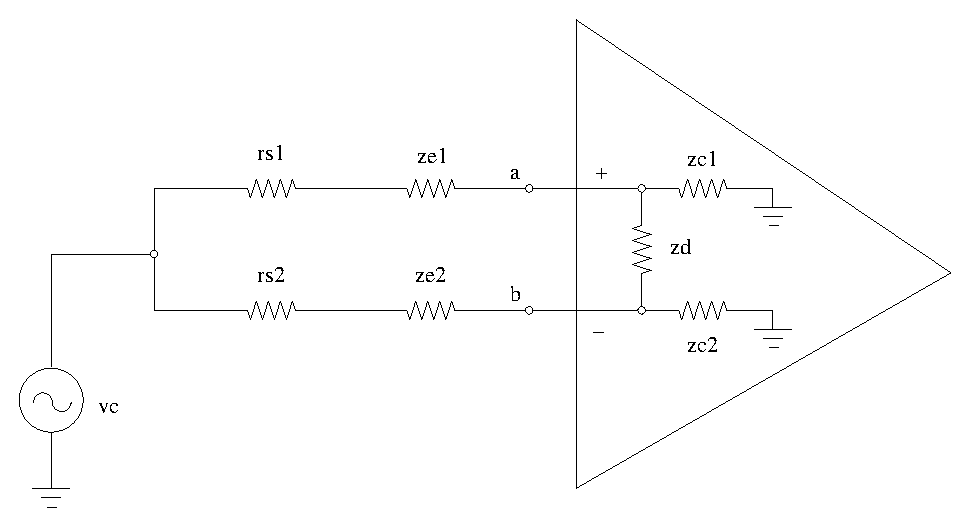
\includegraphics[width=\textwidth]{diff-amp-frontend.eps}
	\caption{ Differential amplifier input}
	\label{fig:diff-amp-frontend}
	\end{center}
\end{figure}

Figure~\vref{fig:diff-amp-frontend} represents the EEG signal path
from the skin surface to the inputs of a differential
amplifier. Figure~\vref{fig:diff-amp-frontend} extends
Figure~\vref{fig:sme-eq} to include the input impedances of the
receiving amplifiers front end. $Z_{e1}$ and $Z_{e2}$ are electrode
impedances, $Z_{c1}$ and $Z_{c2}$ are the common mode amplifier
impedances and $Z_d$ the differential mode amplifier impedance. Any
difference between either $R_{s1}$ -- $R_{s2}$, $Z_{e1}$ -- $Z_{e2}$
or $Z_{c1}$ -- $Z_{c2}$ translates into a false differential signal
voltage over $Z_d$. In commercial instrumentation amplifier (IA)
packages, $Z_{c1}$ and $Z_{c2}$ are usually the non--inverting inputs
of balanced on--chip operational amplifiers. Because the input
impedances of the buffer amplifiers used in IA's are very high the
erroneous differential signal introduced by variations between the
impedance pairs $Z_{c1}$ -- $Z_{c2}$ and $R_{s1}$ -- $R_{s2}$ are
greatly reduced \cite{buffer}.

Due to the low order of EEG signals (1--100~$\mu$Vpp at 0.1--35~Hz)
at the cranial surface) \cite{intro-to-bio} and the fact that
unprepared skin surfaces are used, all possible precautions to prevent
EEG signal attenuation and noise contamination is considered and
implemented where possible.

If the input impedance of the electrode is very high ($>$10M~$\Omega$)
and the output impedance very low ($<$1~$\Omega$) the active electrode
acts as a impedance transformer negating the need for surface
preparation \cite{active-electrode-ca}. The active electrode must be
AC coupled in order to remove electrode offset potentials and allow for
a high gain differential stage in the low level signal processing
module \cite{buffer}.

\subsubsection{Active electrode circuit design and analysis}
\begin{figure}[htbp]
	\begin{center}
	\psfrag{+}{+}		
	\psfrag{-}{--}		
	\psfrag{a}{$a$}		
	\psfrag{b}{$b$}		
	\psfrag{v1}{$v_i$}		
	\psfrag{vo}{$v_o$}		
	\psfrag{c2}{$C_2$}		
	\psfrag{r1}{$R_1$}		
	\psfrag{r2}{$R_2$}		
	\psfrag{c1}{$C_1$}		
	\psfrag{va}{$V_a$}		
	\psfrag{vb}{$V_b$}		
	\psfrag{TL071}[][]{071}
	\includegraphics[]{active-electrode.eps}
	\caption{Active electrode circuit diagram \cite{buffer}}
	\label{fig:active-electrode}
	\end{center}
\end{figure}
The active electrode specification requirements are satisfied by using
a FET--input operational amplifier in the bootstrapped voltage
follower circuit of Figure~\vref{fig:active-electrode} as the active
electrode buffer circuitry.

Capacitor $C_2$ Figure~\vref{fig:active-electrode} decouples any DC
components of the input voltage $v_i$. The inclusion of $C_2$ enables
the active electrode to deliver a AC signal to the differential
amplifier inputs of the low level signal processing module. For a
low--noise design it is important to have the highest gain possible
concentrated in the first amplifier stage of the system
\cite{buffer}. If the applied signals have no DC offsets the
differential stage gain may be set to 60~dB or more without amplifier
saturation problems. The inclusion of $C_2$ makes the addition of a
bias current path mandatory. The bias path can compromise the high
input impedance of the operational amplifier input, negating the
primary benefit of using a operational amplifier as active
electrode. The inclusion of $C_1$ in the bias path enables $R_1$ to
act as a high impedance current source to $v_i$ restoring the input
impedance. Reducing the value of $C_2$ because it feeds a
high-impedance load may lead to unwanted peaks in the AE frequency
response, distorting the measured EEG signal, \cite[p183-184]{art}.

\subsubsection{Active electrode transfer function}
The transfer function of the active electrode circuit of
Figure~\vref{fig:active-electrode} is deduced by summing currents at
nodes $a$ and $b$ and noting the closed loop voltage gain.
\begin{equation}
	\frac{V_a - V_b}{R_1} + \frac{V_a}{R_2} = (v_o - V_a)sC_1
	\label{eq:node-a}
\end{equation}
\begin{equation}
	(V_b - v_i)sC_2 = \frac{V_a - V_b}{R_1}
	\label{eq:node-b}
\end{equation}
With $A_o >> 1$ the open loop gain of the operational amplifier and
$\omega_a$ the corner frequency:
\begin{equation}
	\frac{(V_b - v_o)A_o\omega_a}{s + \omega_a} = v_o
	\label{eq:gain}
\end{equation}
The time constants are defined as follows:
\begin{equation}
	\tau_1 = \frac{R_1\/R_2}{R_1 + R_2}C_1
	\label{eq:tau1}
\end{equation}
\begin{equation}
	\tau_2 = (R_1 + R_2)C_2
	\label{eq:tau2}
\end{equation}
\begin{equation}
	\tau_m = R_2\/C_2
\end{equation}
\begin{equation}
	\tau_a = \frac{1}{\omega_a}
\end{equation}
\begin{equation}
	\tau^2_n = R_1\/R_2\/C_1\/C_2 = \tau_1\/\tau_2
\end{equation}
The active electrode transfer function in terms of input and output
signal voltage is:
\begin{equation}
	\frac{v_o(s)}{v_i(s)} = 
	\frac{s\tau_2(1 + \frac{\tau_1}{s})}{1 + s[\tau_2 + \frac{\tau_m +
	\tau_a}{A_o}] + s^2[\tau^2_n + \frac{\tau_a(\tau_m + \tau_2)}{A_o}] +
	s^3\frac{\tau^2_n\tau_a}{A_o}}
	\label{eq:trans}
\end{equation}

From Equation~\ref{eq:trans} can be seen that the active electrode is
a unity gain voltage follower only at low frequencies excluding
DC. Equation~\ref{eq:trans} can be simplified for low frequencies by
choosing time constant values reducing all terms containing $A_o$ to
insignificant values. For frequencies below the $A_o$ containing terms
in the transfer function denominator the active electrode transfer
function is reduced to:

\begin{equation}
	H(s) = \frac{v_o(s)}{v_i(s)} = \frac{s(s+\frac{1}{\tau_1})}{s^2 +
	\frac{s}{\tau_1} + \frac{1}{\tau_1\/\tau_2}}
\label{eq:simp-trans}
\end{equation}
The damping factor $\epsilon$ for $H(s)$ is given by : 
\begin{equation}
	\epsilon = \frac{(\tau_1/\tau_2)^\frac{1}{2}}{2}
\end{equation}

\begin{figure}[htbp]
	\begin{center}
	\psfrag{tau1}{$\tau_1$}		
	\psfrag{tau2}{$\tau_2$}		
	\psfrag{eps}{$\epsilon$}		
	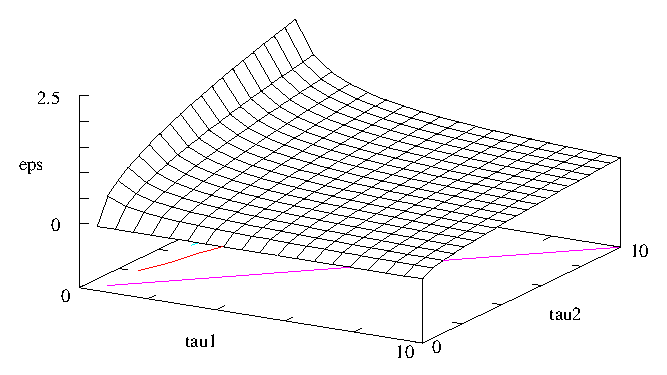
\includegraphics[width=\textwidth]{damping.eps}
	\caption{$\epsilon(\tau_1, \tau_2)$}
	\label{fig:damping}
	\end{center}
\end{figure}

Figure~\vref{fig:damping} plots the damping factor $\epsilon$ as a
function of the time constants $\tau_1$ and
$\tau_2$. Figure~\vref{fig:damping} illustrates the damping factors
greater variance with respect to $\tau_2$ for relatively low $\tau_1$
values. In order to reduce overshoot at $\omega_n$ to acceptable
levels $\tau_1$ and $\tau_2$ values must result in a moderate
$\epsilon$ surface slope.


The natural frequency $\omega_n$ is:
\begin{equation}
	\omega_n = (1/\tau_1\/\tau_2)^\frac{1}{2} = 1/\tau_n
	\label{eq:wn}
\end{equation}

\begin{figure}[htbp]
	\psfrag{tau1}{$\tau_1$}		
	\psfrag{tau2}{$\tau_2$}		
	\psfrag{wn}{$\omega_n$}		
	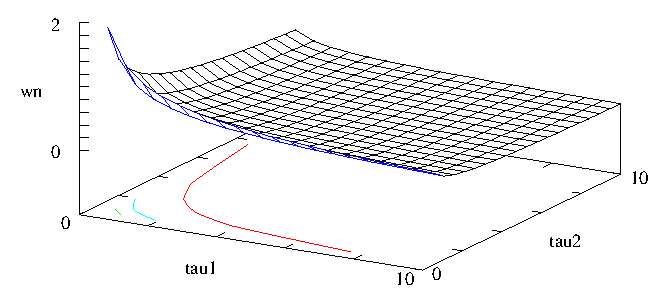
\includegraphics[width=\textwidth]{natural.eps}
	\caption{$\omega_n(\tau_1, \tau_2)$}
	\label{fig:natural}
\end{figure}

Figure~\vref{fig:natural} plots the natural frequency $\omega_n$ as a
function of the time constants $\tau_1$ and $\tau_2$.

The active electrode acts as a high--pass filter for low frequencies,
the amount of overshoot at the natural frequency $\omega_n$ is
determined by the damping factor $\epsilon$.  $\tau_1$ and $\tau_2$
are specified by the values of $C_2$, $C_1$, $R_1$ and $R_2$, see
Equations~\ref{eq:tau1} and \ref{eq:tau2}. The frequency response in
the band of interest must be flat within $\pm$0.5~dB over the
0.1~--~35~Hz range.

Input impedance must remain high and the effect of $\tau_1$ and
$\tau_2$ on the active electrode input impedance must be understood
before specifying time constant values.

\subsubsection{Active electrode input impedance}
Noting the signal current flowing into $C_2$ the active electrode
impedance can be described as follows:
\begin{equation}
	Z = \frac{v_i}{(v_i - v_b)C_2s}
	\label{eq:z}
\end{equation}

Substituting the current Equations~\ref{eq:node-a} and \ref{eq:node-b}
into Equation~\ref{eq:z} and discarding high--frequency terms:
\begin{equation}
	Z = \frac{1 + s\tau_2^2 + s^2\tau_1\/\tau_2}{C_2s}
	\label{eq:z-long}
\end{equation}
substituting $\tau_1$ and $\tau_2$ with the component constants
yields:
\begin{equation}
	Z = \frac{1}{C_2s} + R_1 + R_2 + sR_1R_2C_1
	\label{eq:z-long2}
\end{equation}


\subsubsection{Design for optimal $\tau_1$ and $\tau_2$}
A active electrode must have a high input impedance as well as a flat
frequency response over the band of interest. $\tau_1$ and $\tau_2$
must therefore be designed to ensure that the overshoot at the natural
frequency $\omega_n$ and the attenuation at the low frequency side
does not go beyond the $\pm$0.5~dB specification.

To ensure a high input impedance for interference frequencies it is
necessary to design the electrode's transfer function to act
inductively in the interference frequency range. In general:
\begin{equation}
	R_1 + R_2 < \omega_{int}R_1R_2C_1
	\label{eq:wint}
\end{equation}
$\omega_{int}$ is the interference frequency signal. The modulus of
the transfer function $ \left | H(s) \right | = \left |
\frac{v_o(s)}{v_i(s)} \right | = 1$, at the frequency $\omega_l =
\frac{\omega_n}{\sqrt{2}}$. The same holds for frequencies larger than
the natural frequency $\omega_n$. The lowest frequency in the band of
interest must therefore not be below that of $\omega_l$.

The maximum amplitude of the transfer function $H(s)$ occurs at the
frequency $\omega_{max}$:
\begin{equation}
	\omega_{max} = \frac{\omega_n\sqrt{1 + \sqrt{1 +
	8\epsilon^2}}}{\sqrt{2}}
	\label{eq:omega-max}
\end{equation}
Substituting Equation~\ref{eq:omega-max} into the modulus of the
transfer function yields:
\begin{equation}
	\left | \frac{v_o(s)}{v_i(s)} \right | ^2 = \frac{1 + 8\epsilon^2 +
	(4\epsilon^2 + 1)\sqrt{1 + 8\epsilon^2}}{1 + 8\epsilon^2 +
	(4\epsilon^2 - 1)\sqrt{1 + 8\epsilon^2}}
	\label{eq:max-mag}
\end{equation}

Equation~\ref{eq:max-mag} describes the maximum magnitude of the
transfer function at a specified damping factor $\epsilon$. The
magnitude of the overshoot ($\xi$) is the root of the maximum
magnitude - 1:
\begin{equation}
	\xi = \left | \frac{v_o(s)}{v_i(s)} \right | - 1
	\label{eq:overshoot}
\end{equation}

The rate of attenuation below $\omega_l$ is influenced by
$\epsilon$. The -3~dB frequency $\omega_{-3~dB}$ for $H(s)$
at a specified $\epsilon$ is:
\begin{equation}
	\omega_{-3dB} = \omega_n\sqrt{\sqrt{(2\epsilon^2 + 1) + 1} -
	(2\epsilon^2 + 1)}
	\label{eq:wm1}
\end{equation}

\begin{figure}[htbp]
	\begin{center}
	\psfrag{eps}{$\epsilon$}		
	\psfrag{-3db}{$\omega_{-3dB}$}		
	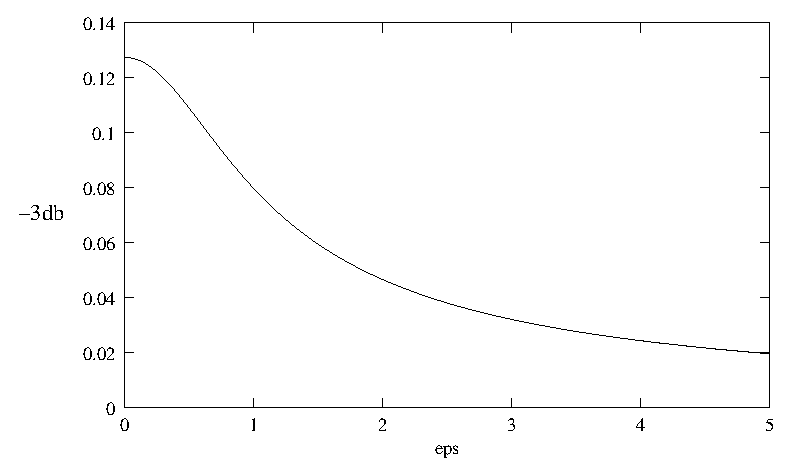
\includegraphics[width=\textwidth]{3db.eps}
	\caption{$\omega_{-3dB}(\epsilon)$}
	\label{fig:3db}
	\end{center}
\end{figure}

Figure~\vref{fig:3db} describes the system roll--off dependency on the
damping factor $\epsilon$. As $\epsilon$ increases the half--power
frequency $\omega_{-3dB}$ decreases. The time constant values must be
chosen to keep $\epsilon$ as small as possible while keeping the
pass--band overshoot within the $\pm$0.5~dB margin.

\subsubsection{Component value calculations}
\label{section:comp-values}
Applying the design equations described in the previous sections
allows for the effective selection of the active electrode component
values.

\begin{table}
\begin{center}	
	\begin{tabular}[htpb]{|c|c|c|c|} \hline
	Parameter & Value \\ \hline
	Minimum input impedance at 50~Hz & 100~M$\Omega$ \\
	Maximum resistor value & 10~M$\Omega$ \\ 
	$f_c$ & 0.1~Hz \\
	\hline
	\end{tabular}
	\caption{AE component specification parameters}
	\label{table:ae-specs}
\end{center}	
\end{table}

With the interference frequency $f_i$~=~50~Hz Equation~\ref{eq:wint}
becomes:

\begin{equation}
	R_1R_2C_1 = \frac{10^8}{100\pi} 
\end{equation}

From Equation~\ref{eq:wn} and $\omega_l = \frac{\omega_n}{\sqrt{2}}$
follows that:
\begin{equation}
	R_1R_2C_1C_2 = \frac{1}{2(0.2\pi)^2} = 1.267 
\end{equation}

For maximum attenuation below 0.1~Hz from Equation~\ref{eq:wm1}
$\epsilon$ must be 1.82. From the definition of $\epsilon$:
\begin{equation}
 	\epsilon =
	\frac{\sqrt{\frac{\tau_2}{\tau_1}}}{2}
\end{equation}
and the preceding equations the active electrode component values can
be calculated. Table~\vref{table:ae-val} is a summary of the component
values used in the realization of the active electrodes. These values
are identical to those specified in \cite{buffer} as the frequency
range is almost identical.

\begin{table}
\begin{center}	
	\begin{tabular}[htpb]{|c|c|} \hline
	Component & Value  \\ \hline
	$C_2$ & 2~$\mu$F \\
	$C_1$ & 680~nF \\ 
	$R_1$ & 680~k$\Omega$ \\
	$R_2$ & 680~k$\Omega$ \\
	\hline
	\end{tabular}
	\caption{Active Electrode component values}
	\label{table:ae-val}
\end{center}	
\end{table}

\section{SAM noise analysis}
\label{section:noise-analysis}
The various active and passive components used in the realization of
the signal acquisition module all contribute to system noise. Each
component acts as either a Shot, Thermal or Flicker noise generator
\cite[p2]{noise-analysis}. The internal noise contributed by the
system components constitutes the ultimate limitation on the signal
acquisition module's resolution \footnote{Analog Dialog,
http://www.analog.com/}.

The lowering of the system signal to noise ratio may lead to the
swamping of low amplitude $\alpha$, $\beta$ and $\gamma$ EEG
components negating the gains won by applying a active electrode for
signal acquisition.

It is prudent to note the relative contribution of system noise by
every system component. Reducing or eliminating factors contributing
to system noise enhances overall system quality and enables the design
to allow for concessions when the noise budget allows it. The SAM
noise analysis concentrates on the system noise introduced by the
active electrode circuit components.


\subsection{Noise types}
To facilitate the process of system noise analysis the definitions of
the most prevalent noise types encountered in the active electrode
circuitry are briefly noted:

\begin{itemize}
	\item\textbf{Shot noise} is associated with current flow and is
	the result of charges crossing a potential barrier. The
	instantaneous current $i$ is therefore the sum of a large number
	of independent random current pulses with a average value of
	$i_{A}$. Shot noise is described as the mean-square deviation from
	the average value for a specified bandwidth. The active electrode
	operational amplifier is the only source of shot noise in the
	active electrode circuit. A low-noise device such as the TL071
	will be employed as the active amplifier.

	\begin{equation}
		\overline{i_S^2} = \overline{i - i_A} = \int{2qi_Adf}
	\end{equation}

	With $df$ the differential frequency and $q$ the electron
	charge. Shot noise has a uniform power density independent of
	temperature. $qi_{A}$ [$\frac{A^2}{Hz}$], the current power
	density is normally used to specify device Shot noise values.

	\item\textbf{Thermal noise} is present in all passive resistive
	elements and is caused by the addition of thermal energy to a
	conductor. Thermal noise is independent of current flow and
	spectrally flat. The mean-square average value of thermal noise
	can be modeled as either a current or a voltage source:

	\begin{equation}
		\overline{e_T^2} = \int{4kTRdf}
		\label{eq:noise-thermal}
	\end{equation}
	\begin{equation}
		\overline{i_T^2} = \int{\frac{4kT}{R}df}
	\end{equation}

	With $df$ the differential frequency, $k$ Boltzmann's constant,
	$T$ absolute temperature [Kelvin] and
	$R$~[$\Omega$]. $4kTR$~[$\frac{V^2}{Hz}$] and
	$\frac{4kT}{R}$~[$\frac{A^2}{Hz}$] are usually noted in a device's
	specification sheet. The largest contributions of thermal noise
	are the resistive components in the AE circuit. In order to curb
	the addition of thermal noise to the system the lowest possible
	resistors are used.

	\item\textbf{Flicker noise} or $\frac{1}{f}$ noise is present in
	all active devices and is associated with DC currents. Flicker
	noise is also found in carbon composition resistors where it is
	usually summed with the device's thermal noise. The average
	mean-square current and voltage values are:
	
	\begin{equation}
		\overline{e_F^2} = \int{\frac{K_e^2}{f}df}
	\end{equation}
	\begin{equation}
		\overline{i_F^2} = \int{\frac{K_i^2}{f}df}
	\end{equation}


	With $K_e$~[V]and $K_i$~[A] are device constants, f~[Hz] frequency
	and $df$ differential frequency. If device current is kept low,
	thermal noise will dominate and the device will not contribute to
	the system flicker noise level. A device's
	$\frac{K_e^2}{f}$~[$\frac{V^2}{Hz}$] or
	$\frac{K_i^2}{f}$~[$\frac{A^2}{Hz}$] noise power density is
	usually noted on it specification sheet.	
\end{itemize}


\subsection{Noise type characteristics}
Thermal and shot noise have Gaussian probability density functions
\cite[p4]{noise-analysis}. With $\delta$ the standard deviation 
of a Gaussian distribution the instantaneous value of a noisy signal is
the signal mean $\pm\delta$ 68\% of the time for any arbitrary signal
sample. The signal variance $\delta^2$ is the average mean-square
variation from the average signal value. For noisy Gaussian signals the
RMS noise value is the standard deviation $\delta$ and the average
mean-square variation around the average value ($\overline{e^2},
\overline{i^2}$) is $\delta^2$ \cite[p4]{noise-analysis}.


The average mean square value of a sum of separate independent noise
sources is the sum of the individual mean square values:
\begin{equation}
	E_{RMS} = \sqrt{e_{1RMS}^2 + e_{2RMS}^2 + ... +e_{nRMS}^2}
	\label{eq:noise-rms}
\end{equation}

The probability of a noise amplitude exceeding $\pm$3$\delta$ is
approximately 0.3\%. To ensure that a noise signal is within
peak-to-peak limits 99.7\% of the time a system must be designed with a
peak-to-peak noise specification 6x the RMS value, that is:
\begin{equation}
	E_{pp} = 6E_{RMS}
	\label{eq:noise-pp}
\end{equation}

The input noise of an operational amplifier contains both white and
$\frac{1}{f}$ noise \cite[p7]{noise-analysis}. The frequency where
white noise equals the $\frac{1}{f}$ noise is referred to as the noise
corner frequency $f_{nc}$.

The average mean-square white noise voltage is a bandwidth dependent
value. Assuming brick-wall pass-bands the following system noise
relationships holds:
\begin{equation}
	\overline{e^2} = \int_{f_l}{f_h}Cdf = C(f_h - f_l) 	
	\label{eq:noise-white}
\end{equation}
With $C$~[$\frac{P}{Hz}$] the spectral power density constant. $C$ is
calculated by squaring the data sheet specified noise value $e_{spec}$
For a $\frac{1}{f}$ noise source the average mean square voltage is:
\begin{equation}
	\overline{e^2} = \int_{f_l}{f_h}\frac{K^2}{f} = K^2ln(\frac{f_h}{f_l}) 	
	\label{eq:noise-1f}
\end{equation}
With $K$~[V] a device constant usually available from the product's
data sheet.

From Equations~\ref{eq:noise-white} and \ref{eq:noise-1f} follows
that:
\begin{equation}
	\frac{K^2}{f_{nc}} = C	
\end{equation}
Adding Equations~\ref{eq:noise-white} and \ref{eq:noise-1f} produces a
equation for the total average mean square noise:

\begin{equation}
	\overline{E^2} = C(f_{nc}ln\frac{f_H}{f_L} + f_{H} - f_{L})
	\label{eq:noise-tot}
\end{equation}

The noise corner frequency ($f_{nc}$) can be determined from the
$nV\sqrt{Hz}$~vs~$f$ graph specified in the active device's product
data sheet. At $f_{nc}$ the white ($n_{white}$)and $\frac{1}{f}$ noise
are equal, $f_{nc}$ is therefore the frequency at which the device
noise equals $\sqrt{2}n_{white}$.

$f_{nc}$ may also be determined by by calculating the value of $K^2$
and dividing by the square of the data sheet noise figure $e_{spec}$:
\begin{equation}
	f_{nc} = \frac{(e_{l}^2 + e_{spec}^2)f_l}{e_{spec}^2}
\end{equation}

In order to apply Equations~\ref{eq:noise-white}, \ref{eq:noise-1f}
and \ref{eq:noise-tot} for realistic noise bandwidth calculations a
equivalent noise bandwidth (ENB) is adapted. For high-order low-pass
filters $f_c$ approaches ENB and no scaling factor is applied
\cite[p10]{noise-analysis}.

\subsection{AE noise analysis}
\label{section:noise-analyses}
\begin{figure}[htbp]
	\begin{center}
    \psfrag{noiseless}{noiseless}
    \psfrag{op-amp}{op-amp}	
	\psfrag{a}{a}						
	\psfrag{c2}{$C_2$}		
	\psfrag{c1}{$C_1$}		
	\psfrag{r1}{$R_1$}		
	\psfrag{r2}{$R_2$}		
	\psfrag{Et}{$\overline{E_t}$}		
	\psfrag{en}{$\overline{e_{int}}$}		
	\psfrag{i+}{$\overline{i_p}$}		
	\psfrag{i-}{$\overline{i_n}$}		
	\psfrag{e1}{$\overline{e_{R_1}}$}		
	\psfrag{e2}{$\overline{e_{R_2}}$}		
	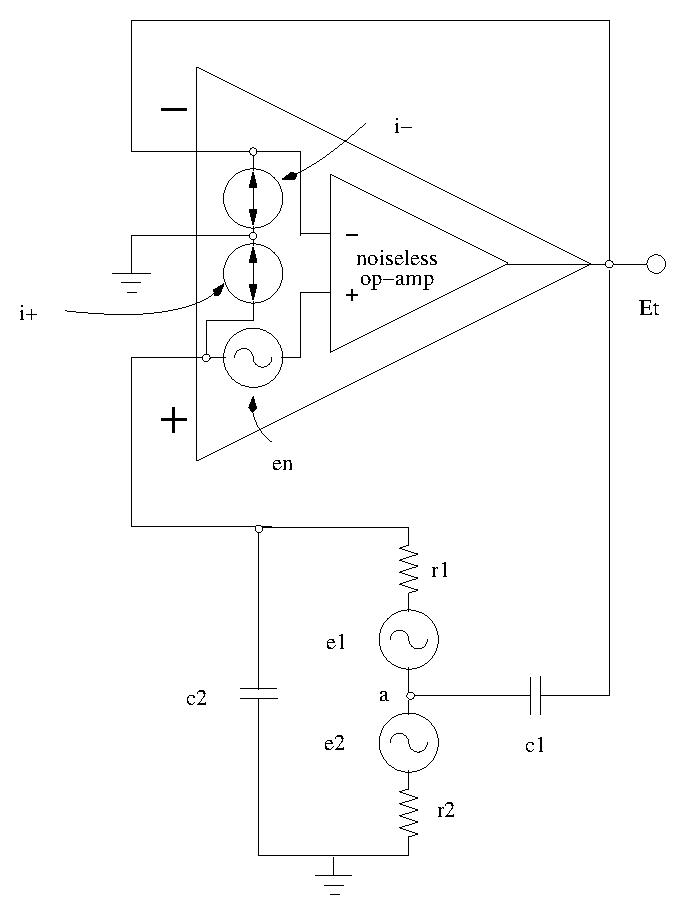
\includegraphics{ae-noise-eq.eps}
	\caption{Active electrode equivalent noise circuit.}
	\label{fig:ae-noise-eq}
	\end{center}
\end{figure}

Random noise sources in operational amplifiers are generally referred
to the amplifier input. The equivalent noisy amplifier are modeled as
a group of uncorrelated noise generators in series and parallel with
the inputs of a noiseless operational amplifier
\cite[11]{noise-analysis}. 

Figure~\vref{fig:ae-noise-eq} depicts the equivalent active electrode
noise circuit of Figure~\vref{fig:active-electrode}. In the equivalent
circuit the signal input is grounded and five noise sources are added:
\begin{itemize}
	\item A internal voltage noise source $\overline{e_{int}}$ referred
	to the non-inverting amplifier input.

	\item Two Johnston noise sources $\overline{e_{R_1}}$ and
	$\overline{e_{R_1}}$ contributed by $R_1$ and $R_2$.

	\item Two internal current noise sources $\overline{i_n}$ and
	$\overline{i_p}$ alternatively referred to the inverting and
	non-inverting amplifier inputs.

\end{itemize}

\subsubsection{Equivalent noise circuit analysis}
The principle of superposition may be applied due to the uncorrelated
nature of the individual noise sources. A single noise source is
isolated and all other sources ignored. By applying standard circuit
analysis techniques the system noise generated by a single source is
calculated. This procedure is followed for all noise sources and the
total noise value calculated by applying Equation~\ref{eq:noise-rms}.


The average value $\overline{E_{R_1}}$ is determined by disregarding
all noise sources except $R_1$ and summing the currents away from node
$a$ in Figure~\vref{fig:ae-noise-eq}:
\begin{equation}
	\overline{E_{R_1}} = \overline{e_1}(\frac{Z_1}{R_1 + Z_2} +
	\frac{Z_1}{R_2} + 1)
	\label{eq:noise-er1t}
\end{equation}
With $Z_1$ and $Z_2$ the impedances due to capacitors $C_1$ and $C_2$
respectively. To minimize the Johnston noise component the maximum
resistance used in the active electrode must be kept to a minimum,
that is $R_1$ = $R_2$ = $R$ as stated in
Section~\ref{section:comp-values}.
\begin{equation}
	\overline{E_{R_1}} = \overline{e_{R_1}}\left(\frac{Z_1(2R +
	Z_2)}{R(R + Z_2}) \right)
\end{equation}

Squaring the mean value $\overline{e_{R_1}}$ and substituting into the
thermal noise equation (Equation~\ref{eq:noise-thermal}) leads to the
system thermal noise due to $R_1$:
\begin{equation}
		\overline{E_{R_1}}^2 = \overline{e_{R_1}}^2\left (\frac{Z_1(2R +
	Z_2)}{R(R + Z_2)} \right )^2
\end{equation}

\begin{equation}
	\Rightarrow	\overline{E_{R_1}}^2 = 4kTR\int\/\left (\frac{Z_1(2R +
	Z_2)}{R(R + Z_2)} \right )^2df
	\label{eq:noise-therm1}
\end{equation}

Similar reasoning holds for $R_2$:
\begin{equation}
	\Rightarrow	\overline{E_{R_1}}^2 = 4kTR\int\/\left (\frac{Z_1(2R +
	Z_2)}{R(R + Z_2)} \right )^2df
	\label{eq:noise-therm2}
\end{equation}

From Equation~\ref{eq:noise-rms} follows that the total RMS noise
voltage due to the active electrode external resistors is the root sum
of Equations~\ref{eq:noise-therm1} and \ref{eq:noise-therm2}:
\begin{equation}
	E_{RMS} = \sqrt{\overline{E_{R1}^2} + \overline{E_{R_2}^2}}
	\label{eq:noise-rtot1}
\end{equation}
\begin{equation}
	\Rightarrow E_{RMS} = \sqrt{\int \left (8kTR
	\left(\frac{Z_1(2R + Z_1)}{R(R + Z_2)} + 1\right)^2 \right) df}
	\label{eq:noise-rtot2}
\end{equation}

The external resistors are the only devices that can be varied in the
circuit design. The other noise sources are inherent to the active
devices and cannot be manipulated short of choosing the device
according to its published noise specifications.

For this reason the lowest resistor values were chosen that a design
will allow. The TL071 ($v_n = 18~\frac{nV}{\sqrt{Hz}}$)\footnote{TL071
Data sheet} operational amplifier were chosen to implement all active
components of the system excluding the instrumentation amplifier.

\subsection{Physical electrode implementation}
\begin{center}
\begin{figure}[htbp]
	\begin{center}
	\psfrag{x1}{$x_1$}						
	\psfrag{x2}{$x_2$}						
	\psfrag{x3}{$x_3$}						
	\psfrag{x4}{$x_4$}						
	\psfrag{y1}{$y_1$}
	\psfrag{y2}{$y_2$}
	\psfrag{y3}{$y_3$}
	\psfrag{a}{a}
	\psfrag{b}{b}
	\psfrag{c}{c}
	\psfrag{d}{d}
	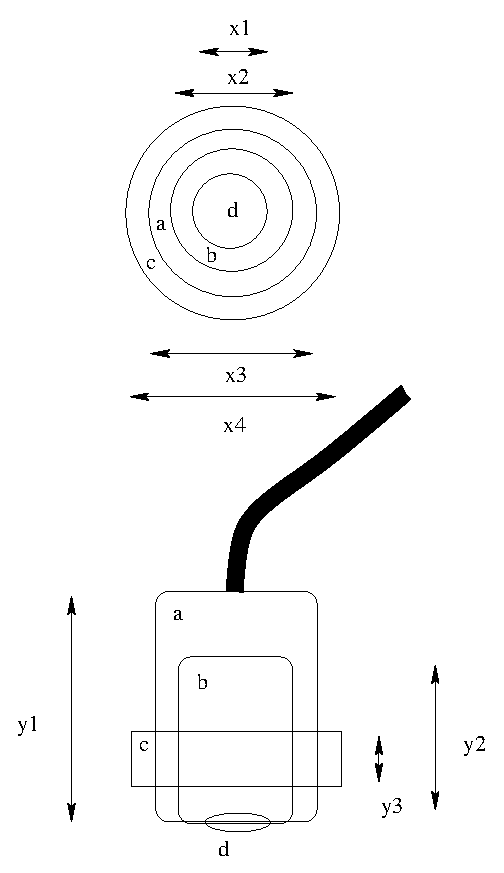
\includegraphics{electrode-imp.eps}
	\caption{Active electrode structural design parameters.}
	\label{fig:electrode-structure}
	\end{center}
\end{figure}
\end{center}

\begin{table}
\begin{center}	
	\begin{tabular}[htpb]{|c|c|} \hline
	Measurement & Value [mm] \\ \hline
	$x_1$ & 13 \\
	$x_2$ & 20 \\ 
	$x_3$ & 25 \\
	$x_4$ & 33 \\
	$y_1$ & 30 \\
	$y_2$ & 20 \\
	$y_3$ & 7 \\
	\hline
	\end{tabular}
	\caption{Active electrode dimensions}
	\label{table:ae-dim}
\end{center}	
\end{table}

Figure~\vref{fig:electrode-structure} depicts the active electrode as
a single physical unit. Table~\ref{table:ae-dim} lists the electrode
dimensions. Casings a,b and c are press--molded vulcanized rubber
plugs available commercially. The active electrode circuitry is
contained in plug b. The passive electrode (d) may be silver--plated
\footnote{The process of Ag--plating is outlined in
Appendix~\ref{appendix:plating} } to reduce contamination noise levels
\cite{electrode-stability}. 

Encapsulating the AE electronics in the electrode body allows for a
neat and manageable device. The encapsulating rubber also acts as a
robust cage, protecting the electronics against impact. The external
electrode housing surface were treated with Graphit\footnote{GRAPHIT,
Kontakt Chemie, CRC Industries, Belgium}, a graphite containing
surface paint. The surface paint aids in the prevention of possible
destructive static build--up on the electrode housing.


\begin{center}
\begin{figure}[htbp]
	\begin{center}
	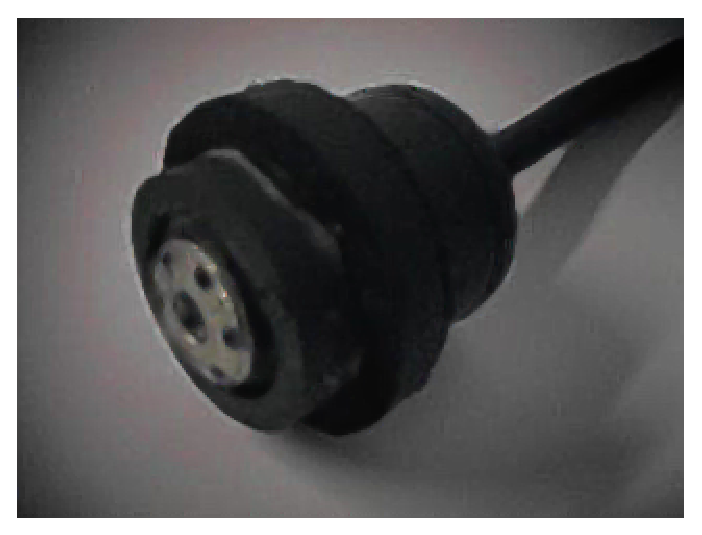
\includegraphics{electrode.ps}
	\caption{Active electrode implementation.}
	\label{fig:electrode-implimentation}
	\end{center}
\end{figure}
\end{center}

Figure~\ref{fig:electrode-implimentation} is a photograph of an active
electrode ('Blue')\footnote{The AE's were labeled 'Blue' and 'Red'}
used in the project. The outer and inner housing as well as the
mounting ring is visible. The inner plug containing the AE electronics
fits into the outer plug with the connecting cable threaded through
the base of the outer plug. The top of the inner plug supports the
passive electrode interface.

During active electrode implementation it was decided to use the
Ag/AgCl metal electrodes embedded in standard ECG gel electrodes as
active electrode tips. The passive electrode was replaced with a clip
that fits most standard ECG electrode fasteners. The clip is visible
at the front of the electrode in
Figure~\ref{fig:electrode-implimentation}.


\subsection{SAM container implementation}
\begin{figure}[htbp]
	\begin{center}
	\psfrag{wool}[][]{Velcro wool}
	\psfrag{hooks}[][]{Velcro hooks}
	\psfrag{x2}[][]{$x_2$}
	\psfrag{x1}[][]{$x_1$}		
	\psfrag{x3}[][]{$x_3$}		
	\psfrag{y1}[][]{$y_1$}
	\psfrag{y2}[][]{$y_2$}
	\psfrag{z}[][]{$z$}
	\psfrag{d}[][]{$d$}
	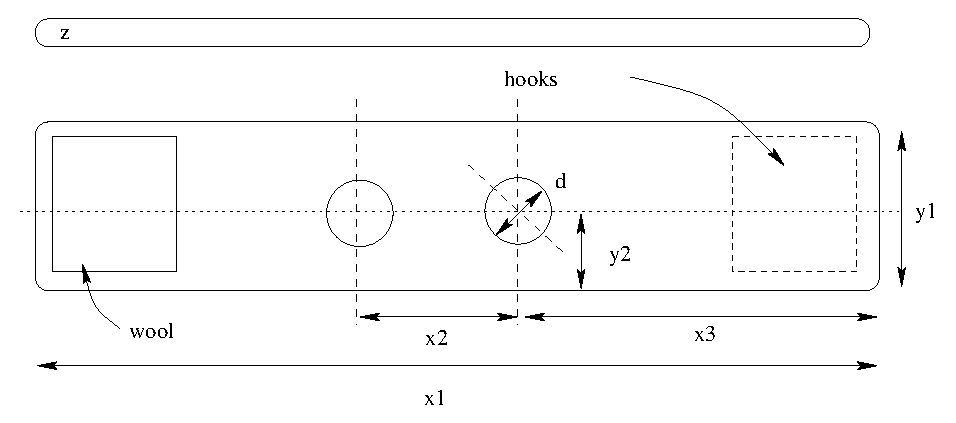
\includegraphics[width=\textwidth]{headband2.eps}
	\caption{SAM container implementation.}
	\label{fig:container}
	\end{center}
\end{figure}

\begin{table}
\begin{center}	
	\begin{tabular}[htpb]{|c|c|} \hline
	Measurement & Value [mm]\\ \hline
	$x_1$ & 670 \\ 
	$x_2$ & 90 \\
	$x_3$ & 280 \\
	$y_1$ & 50 \\ 
	$y_2$ & 25 \\ 
	$d$ & 23 \\ 
	$z$ & 4 \\
	\hline
	\end{tabular}
	\caption{SAM container dimensions}
	\label{table:sam-container}
\end{center}	
\end{table}

Figure~\vref{fig:container} details the SAM container
design. Table~\ref{table:sam-container} lists the SAM container
dimensions. The container resembles a sweat or head--band and is made
using a dense foam rubber strip and Velcro fasteners. The head--band
contains two holes that corresponds to the $F_{p1}$ and $F_{p2}$
montage positions when mounted. The diameter ($d$) of the holes are
slightly less than the diameter of the electrode outer plug, this
ensures a tight and secure fit of the electrode in the head--band.

\begin{center}
\begin{figure}[htbp]
	\begin{center}
	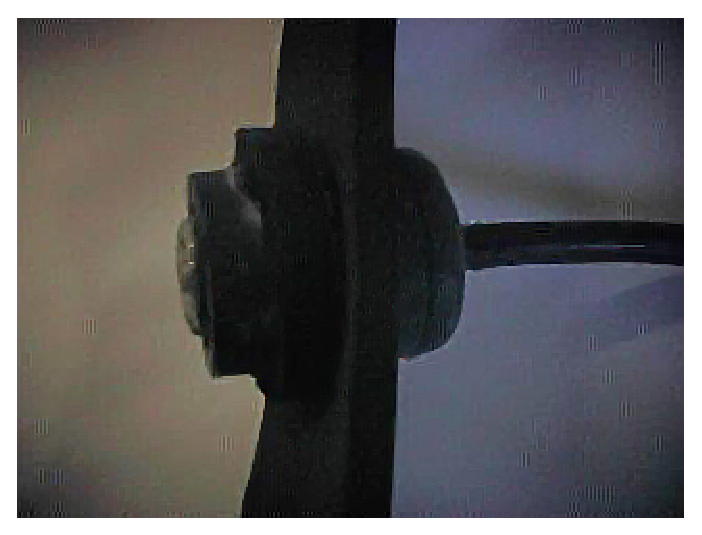
\includegraphics{single-electrode-headband.ps}
	\caption{Head--band mounted electrode.}
	\label{fig:headband-mounted-electrode}
	\end{center}
\end{figure}
\end{center}

Figure~\vref{fig:headband-mounted-electrode} shows an active electrode
mounted on the SAM head--band of Figure~\vref{fig:container}. The
outer plug fits snugly through the head--band hole.  When the
head--band is fastened on the head pressure is applied to the outer
ring and the electrode pressed against the skin. The applied pressure
from the head--band keeps the electrodes firmly in position at their
$F_{p1}$ and $F_{p2}$ positions.


\begin{center}
\begin{figure}[htbp]
	\begin{center}
	\includegraphics{electrode-headband.ps}
	\caption{Head--band mounted electrodes.}
	\label{fig:headband-mounted-electrodes}
	\end{center}
\end{figure}
\end{center}

Figure~\vref{fig:headband-mounted-electrodes} shows both electrodes
mounted in their respective positions. The head--band is positioned in
the same manner as when it is used during normal system operation. The
Electrode cable terminators are visible in the center of the
head--band circle.


\subsubsection{Electrode placement}
\begin{figure}[htbp]
\begin{center}
	\includegraphics*{electrodes-front-headband.ps}
	\caption{Electrodes mounted at $F_{p1}$ and $F_{p2}$}
\label{fig:mount1}
\end{center}
\end{figure}

The electrodes are positioned on the head--band in such a manner that
the electrode placement on the scalp will correspond to the $F_{p1}$
and $F_{p2}$ 10--20 EEG montage positions when the container is
fastened on the head, see Figure~\ref{fig:mount1}. The active
electrode clips are visible in front of the photograph. The Ag/AgCl
electrode tips are clipped unto the electrodes before use. 


\begin{figure}[htbp]
\begin{center}
	\includegraphics*{unmounted-SMEandSAM.ps}
	\caption{Unmounted SAM and SME}
	\label{fig:unSMEandSAM}
\end{center}
\end{figure}

Figure~\ref{fig:unSMEandSAM} shows the SAM container with the attached
electrodes together with the SME physical head module. The $F_{p1}$
and $F_{p2}$ on both the SAM and SME correspond.

\begin{figure}[htbp]
\begin{center}
	\includegraphics*{mounted-SMEanSAM.ps}
	\caption{Mounted SAM and SME}
	\label{fig:SMEandSAM}
\end{center}
\end{figure}

Figure~\ref{fig:SMEandSAM} shows the signal acquisition mounted on the
standard measurement environment head model. During noise and
interference measurements the SAM and SME modules were used in this
configuration. The test--setup of Figure~\ref{fig:SMEandSAM} was
physically moved closer and nearer suspected interference sources
during testing.

The configuration shown in Figure~\ref{fig:SMEandSAM} is the normal
manner in which the SAM is used when measurements on a human subject
is done.

\section{SAM measurements and characterization}

\subsection{Noise and interference measurements}

\begin{figure}[htbp]
\begin{center}
	\psfrag{+}[][]{+}
	\psfrag{-}[][]{-}
	\psfrag{TL071}[][]{TL071}
	\psfrag{s1}[][]{$S_1$}
	\psfrag{vo}[][]{$v_o$}
	\includegraphics*{ae-m.eps}
	\caption{AE noise measurement circuit}
	\label{fig:ae-m}
\end{center}
\end{figure}

Figure~\ref{fig:ae-m} represents the circuit used during the active
electrode noise measurements. Both AE used in the system were
evaluated. Measurements from each AE were very similar and no
distinction between either of the AE's were noticed or reported.
Measurements from only one AE are represented.

For noise measurements switch $S_1$ are either opened or closed. When
evaluating SME signals $S_1$ is always opened.

\begin{figure}[htbp]
\begin{center}
	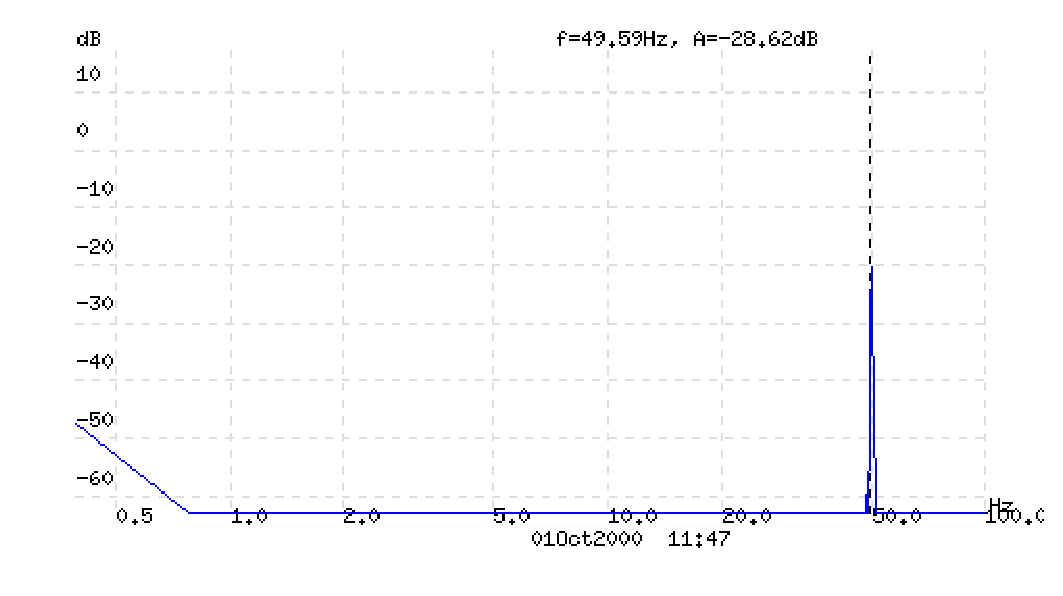
\includegraphics[width=\textwidth]{AE1OF.ps}
	\caption{AE off grounded}
	\label{fig:ae1-n}
\end{center}
\end{figure}
 
Figure~\ref{fig:ae1-n} represents the signal measured at the output of
the grounded ($S_1$ closed) un-powered active electrode. The noise
floor is nominally flat with the -28~dB 50~Hz interference spike the
only relevant feature of the graph. The measurement of
Figure~\ref{fig:ae1-n} and all other measurements note in this section
were done with the 'Blue' AE of
Figure~\ref{fig:electrode-implimentation}. Shielded commercial
oscilloscope probes were used during all measurements, a floating
probe always displayed a -64~dB 50~Hz interference signal, the signal
of Figure~\ref{fig:ae1-n} consists therefore primarily of the
interference coupled into the AE.


\begin{figure}[htbp]
\begin{center}
	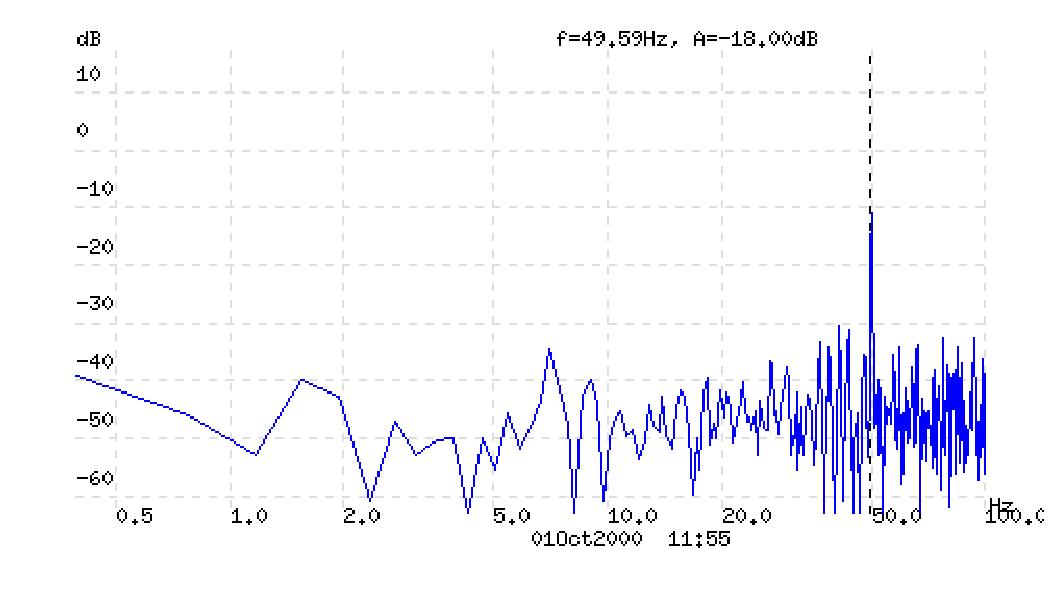
\includegraphics[width=\textwidth]{AE2OFOP.ps}
	\caption{AE off un-grounded}
	\label{fig:ae2-n}
\end{center}
\end{figure}

Figure~\ref{fig:ae2-n} represents the signal measured at the output of
the un-grounded ($S_1$ open) un-powered active electrode. The noise
floor is approximately -20~dB higher than that of
Figure~\ref{fig:ae1-n}. Once more a prominent feature of the graph is
the a -18~dB 50~Hz interference spike. Figure~\ref{fig:ae2-n}
represents the worse case noise scenario for a AE, input noise of this
magnitude will occur when the electrode loses contact with the
subject's skin.


\subsection{SME Measurements}
In order to test the frequency response of the AE the SME test signals
were applied to the AE input. The $100~\mu\/V$ signals from the SME
were to low to register on the test equipment and were raised for the
AE signal tests. Test signals of the magnitude used to test the AE
were very badly clipped even at the AD620 output. For system tests the
SME signals were adjusted to levels that were passed unclipped
throughout the system.


\begin{figure}[htbp]
\begin{center}
	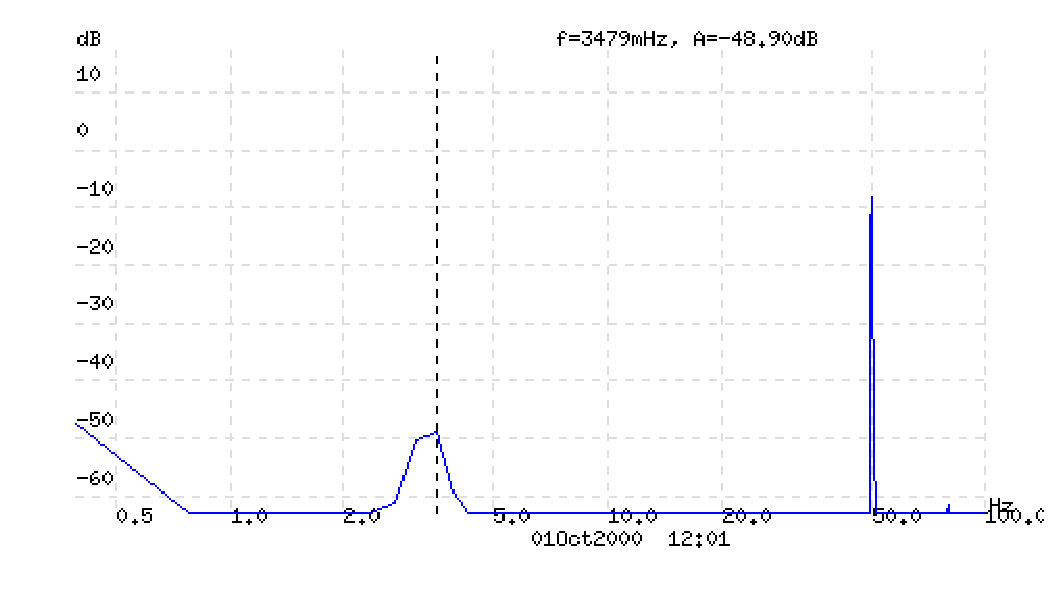
\includegraphics[width=\textwidth]{AE63SME.ps}
	\caption{$\delta$ (3~Hz) signal test}
	\label{fig:ae-sme3}
\end{center}
\end{figure}

Figure~\ref{fig:ae-sme3} represents the signal measured at the output
of the AE while applying a $\delta$ SME test signal at the SME
input. The $\delta$ signal amplitude were set at a visible value of
-50~dB (-48,9~dB measured). The 50~Hz interference signal is markedly
larger ($\pm$15~dB) than that of Figure~\ref{fig:ae1-n}. This is due
to the unshielded signal cables used to carry the test signal from the
SME to the AE.


\begin{figure}[htbp]
\begin{center}
	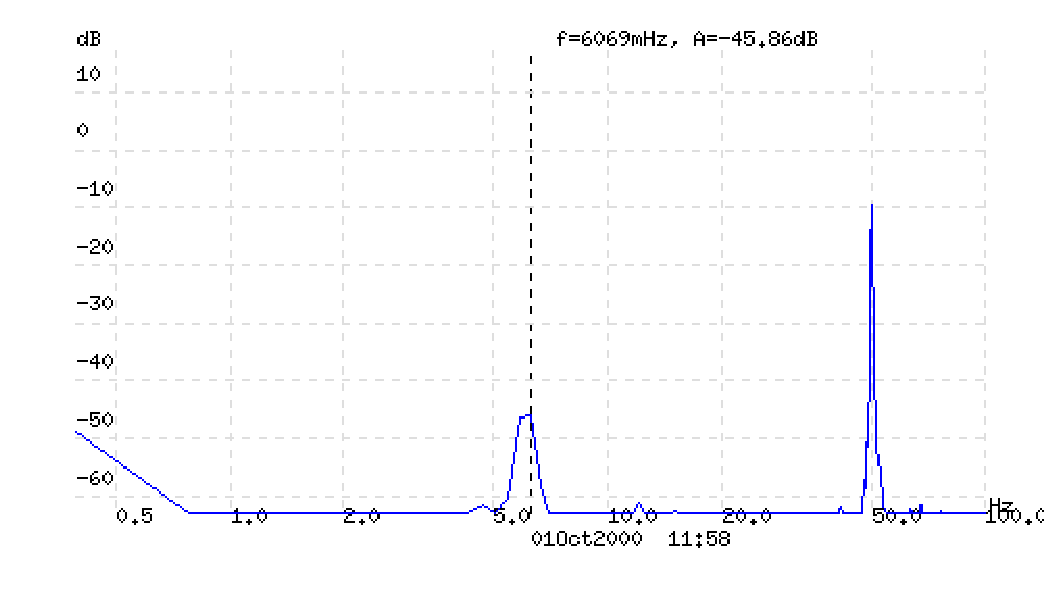
\includegraphics[width=\textwidth]{AE36SME.ps}
	\caption{$\theta$ (6~Hz) signal test}
	\label{fig:ae-sme6}
\end{center}
\end{figure}

Figure~\ref{fig:ae-sme6} represents the signal measured at the output
of the AE while applying a $\theta$ SME test signal at the SME
input. The $\theta$ signal amplitude were set at a visible value of
-50~dB (-45,86~dB measured). The mark at the 6~Hz spike were set
manually and is therefore not completely accurate.

\begin{figure}[htbp]
\begin{center}
	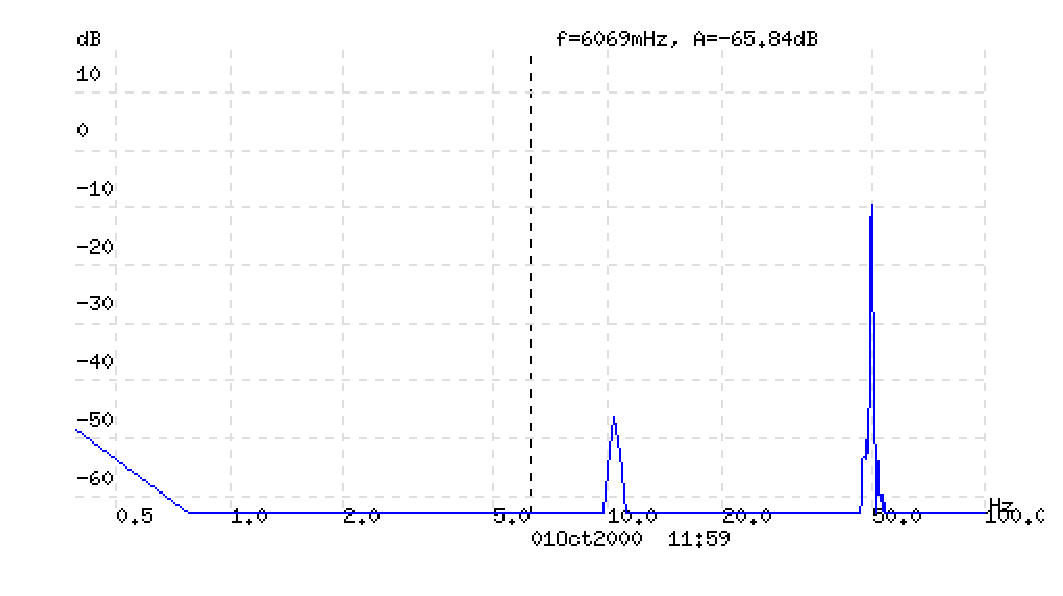
\includegraphics[width=\textwidth]{AE410SME.ps}
	\caption{$\alpha$ (10~Hz) signal test}
	\label{fig:ae-sme10}
\end{center}
\end{figure}

Figure~\ref{fig:ae-sme10} represents the signal measured at the output
of the AE while applying a $\alpha$ SME test signal at the SME
input. The $\alpha$ signal amplitude were set at a visible value of
-50~dB (-49,30~dB measured -- not visible on the graph). Various
points around the 10~Hz peak were tested for signal strength as the
$\alpha$~SME signal is used as the primary test signal during system
tests. The $\alpha$ SME signal has the lowest total harmonic
distortion in the SME test signal suite.


\begin{figure}[htbp]
\begin{center}
	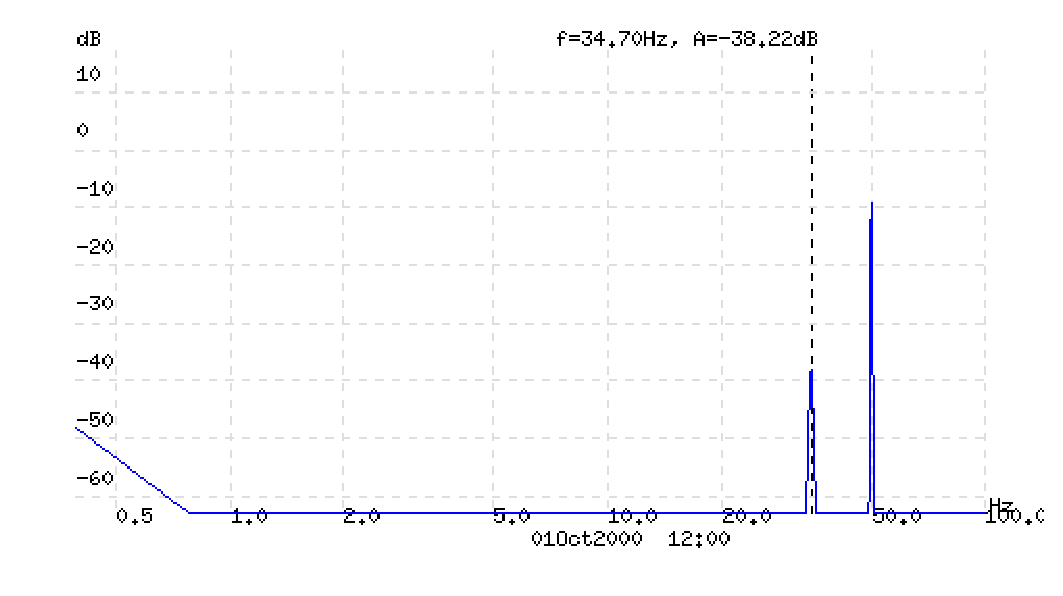
\includegraphics[width=\textwidth]{AE535SME.ps}
	\caption{$\gamma$ (35~Hz) signal test}
	\label{fig:ae-sme35}
\end{center}
\end{figure}

Figure~\ref{fig:ae-sme35} represents the signal measured at the output
of the AE while applying a $\gamma$ SME test signal at the SME
input. The $\gamma$ signal amplitude were set at a visible value of
-50~dB (-38,22~dB measured).

\subsubsection{Measurement conclusion}

The AE were evaluated using SME range of test frequencies. The AE did
not exhibit any unexpected behavior at any of the test
frequencies. The amount of 50~Hz interference present in the shielded
AE is higher than expected. Passive shielding of the AE cabling is not
as effective as was hoped. If time and effort permits a active shield
drive as described in the AD620 data sheet might be investigated.




